\documentclass[11pt]{article}

\usepackage{graphicx}
\usepackage{url}
\usepackage{hyperref}

\begin{document}

\begin{center}
{\Large \bf Building the VMW Raspberry Pi / AY-3-8910 Chiptune Player}\\[2ex]
by Vincent M. Weaver\\[3ex]
\url{http://deater.net/weave/vmwprod/hardware/ay-3-8910/}\\[3ex]
2 June 2017
\end{center}

\begin{center}
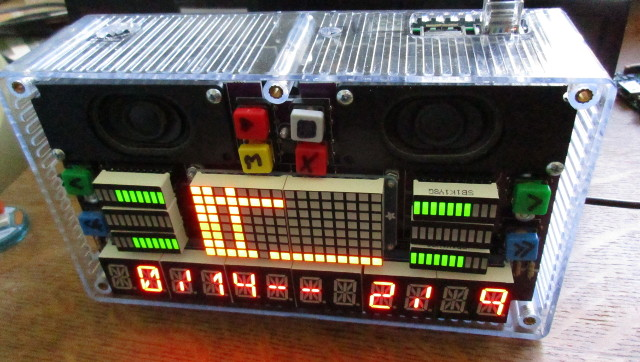
\includegraphics[width=3in]{figs/0377_front_view.jpg}
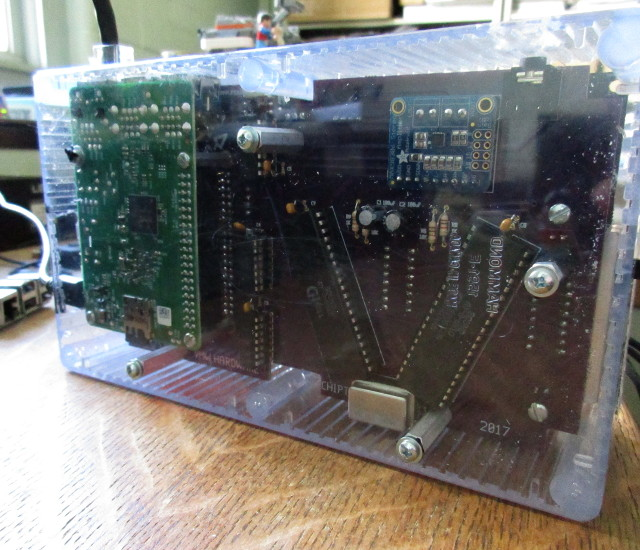
\includegraphics[width=3in]{figs/0378_back_view.jpg}
\end{center}
\vspace{3ex}
\begin{center}
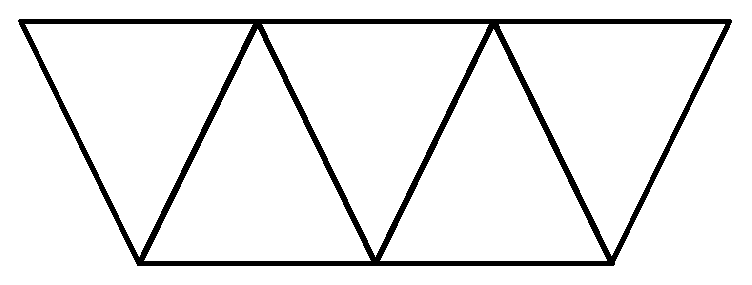
\includegraphics[width=1in]{figs/vmw}\\
A VMW Hardware Production
\end{center}

\pagebreak

\section{Introduction}

This document describes a custom Raspberry-Pi Chiptune Player with
LED visualization.
The design contains an EEPROM and can be considered a Pi ``hat'', although
I have not gotten around to testing or programming the EEPROM interface.

The sound board contains two AY-3-8910~\cite{ay38910} sound chips, a design
dating to the 1980s.
These were popular chips, found in the ZX Spectrum and Atari ST.
I know of them from their appearance on the Apple II Mockingboard soundcard.

Features found on the device:
\begin{itemize}
\item Dual AY-3-8910 for 6-channel stereo sound
\item i2c display including 8x16 display, 6 bargraphs, 12 characters, and 8 buttons
\item i2c real-time-clock so it can be used as an alarm clock
\item 1-wire temperature sensor
\item Dual 4W speakers, can also output to stereo 3.5mm jack
\item ``hat'' EEPROM 
\end{itemize}

%%%%%%%%%%%%%%%%%%%%%%
%%%%%%%%%%%%%%%%%%%%%%
\section{Pi Interface}
%%%%%%%%%%%%%%%%%%%%%%
%%%%%%%%%%%%%%%%%%%%%$

%%%%%%%%%%%%%%%%%%%%%%
\subsection{AY-3-8910}
%%%%%%%%%%%%%%%%%%%%%%

The AY-3-8910 circuit is more or less the one found as a reference
implementation in the manual.

To limit the number of GPIOs needed, two 74HC595 shift registers are used
to provide the parallel inputs to the AY-3-8910.
The Pi drives these via the SPI interface (level shifted up to 5V
by 74AHCT125N chips).

To actually drive the bus signals, three GPIOs are used, hooekd to
!RESET, BDIR1 and BC1 on the AY-3-8910s.

The clocks on the AY-3-8910s are driven by a 1MHz crystal, which seems
to do a reasonable job.
The various 1980s computers used different clock crystals ranging from
1MHz to 2MHz, but with proper scaling of the audio files 1MHz seems
to suffice.

There is a rough hand-drawn schematic shown in Figure~\ref{figure:schematic}.

\begin{figure}[tph]
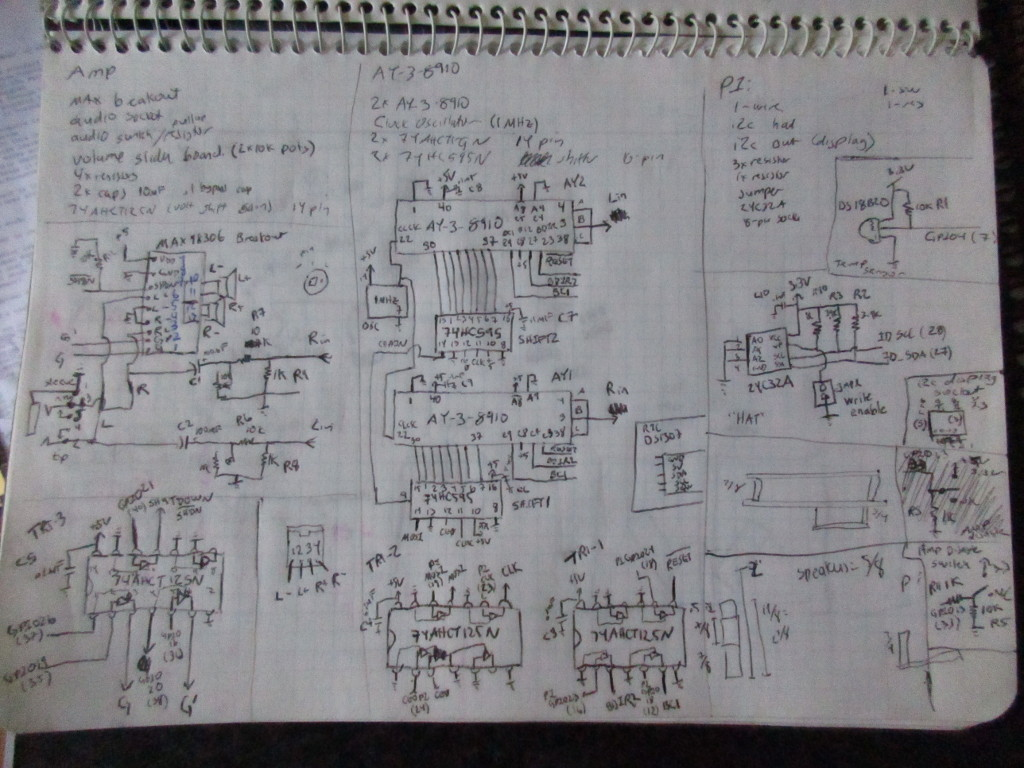
\includegraphics{figs/0380_schematic.jpg}
\caption{Schematic for the sound board.~\label{figure:schematic}}
\end{figure}

%%%%%%%%%%%%%%%%%%%%
\subsection{Display}
%%%%%%%%%%%%%%%%%%%%

The LED displays are driven by the i2c bus.
The 14-segment displays and the 8x16 display are standard breakout boards
from Adafruit.  They have been configured so each has its own 
i2c address.

The bargraphs are hooked up manually to a ht16k33 breakout board, which
is an i2c LED adapter.

The buttons are connected to the ht16k33 breakout via the interface
described in the datasheet~\cite{ht16k33}.

No schematic is available for the Display board, I more or less took the
breadboard design directly into geda/pcb with a long hand-written
netlist.

%%%%%%%%%%%%%%%%%%
\subsection{Audio}
%%%%%%%%%%%%%%%%%%

The audio output from the AY-3-8910 is fed into both a 3.5" stereo
jack, as well as a MAX98306 class-D amplifier breakout board.
The MAX98306 feeds into dual 4 Ohm 3.7W speakers.

The MAX98306 gain can be controlled via input pins, which are hooked to
GPIO pins on the raspberry pi (through a 74AHCT125 for 3.3V to 5V
level shifting).

This works, but the output on the speakers is often
too loud even with the lowest
gain setting.
Because of this two 10k sliding potentiometers were used to act as analog
volume controls.

There is a SPDT slide switch to indicate to the Pi that you want to disable
the speakers.
This is all in software; it is up to the Pi to monitor the GPIO and turn
off the speakers in hardware.

I spent a lot of time trying to design a circuit that could detect the
impedeance of the jack and automatically cut off the speakers when a
plug is inserted.
I could not get this to work.

The Pi can shutdown the amplifier using a GPIO line connected to the
!SHDN signal.
A pull-down resistor is in place to make sure this signal is pulled low
until the Pi gets around to driving it.

%%%%%%%%%%%%%%%%%%%%%%%%
\subsection{Peripherals}
%%%%%%%%%%%%%%%%%%%%%%%%

While designing the board, various extra features were added.

A DS18B20 1-wire temperature sensor was added to monitor for overheating.
It is unclear if extra ventilation holes will be needed in the case.

An EEPROM was connected to the Pi i2c-configuration bus.
This could be used to autoconfigure the device as a ``hat'' although
I have not tested this functionality.

A DS1307 i2c Real Time Clock was added, so that the Pi can remember
the time when disconnected from the internet.
This could allow use in alarm-clock type situations.


%%%%%%%%%%%%%%%%%%%%%%
%%%%%%%%%%%%%%%%%%%%%%
\section{Performance}
%%%%%%%%%%%%%%%%%%%%%%
%%%%%%%%%%%%%%%%%%%%%$

The device functions more or less well when being run by a 
Raspberry Pi-2B.

I tried using a Pi-B+ but it was not able to run things smoothly.
Likely Linux was interrupting and messing up the real time handling
(especially when I am logged in over the ethernet at the same
time doing debugging).

To play a ym5 file you need to update the 14 registers every 50Hz
(20ms).

The traditional /sys GPIO interface for Linux is much too slow for this.
Instead I use the bcm2835 library~\cite{bcm2835}.

The original implementation did not use SPI, but bitbanged the GPIOs.

\begin{tabular}{|c|c|}
\hline
Routine	& Time (ms) \\
\hline
\hline
ym\_play\_frame (gpio) & 14ms \\
\hline
display\_update (i2c) & 1-3ms \\
\hline
display\_keypad\_read: & 0.5ms \\
\hline
display\_string       & 5ms \\
\hline
\end{tabular}

As you can see, it could sometimes overflow the 20ms window.
Displaying a string on the 14seg displays takes especially a long time
as the 3 subdisplays are each on a separate i2c address.

By moving to SPI it reduced ym\_play\_frame to 5ms, allowing
the sound and visualization to happen in the deadline.

There is still some occasional jitter in the output.
The solution might be to move to bare-metal coding (or a real time operating
system) as Linux by default is not configured for real-time use.





%%%%%%%%%%%%%%%%%%
%%%%%%%%%%%%%%%%%%
\section{Software}
%%%%%%%%%%%%%%%%%%
%%%%%%%%%%%%%%%%%%

I provide software that can drive this board on github:\\
\url{https://github.com/deater/vmw-meter.git}

You can download it with:
{\tt git clone https://github.com/deater/vmw-meter.git}
and look in the ay-3-8910 directory.

Software includes a YM5 player, conversion software, a rough tracker
for creating your own chiptunes, and more.



%%%%%%%%%%%%%%%%%%
%%%%%%%%%%%%%%%%%%
\section{Building}
%%%%%%%%%%%%%%%%%%
%%%%%%%%%%%%%%%%%%

%%%%%%%%%%%%%%%%%%%%%%%%%%%%%%%%%%%%%%%%%%%%
\subsection{The Primary Sound Board ``hat''}
%%%%%%%%%%%%%%%%%%%%%%%%%%%%%%%%%%%%%%%%%%%%

\begin{table}[thp]
\caption{Sound Board Parts.~\label{table:sound_parts}}
\centering
\sf
\begin{tabular}{|c|c|c|c|r|r|}
\hline
NAME		& WHERE		& PART\#                  & QTY	& PRICE	   & TOTAL \\
\hline
\hline
PCB		& OSH Park	& VMW-CHIPTUNE-SOUND-MK1  & 1	& \$45.08  & \$45.08 \\
\hline
PCB		& OSH Park	& VMW-CHIPTUNE-SLIDER-MK1 & 1   &  \$2.80  &  \$2.80 \\
\hline
AY-3-8910	& eBay		& AY-3-8910		  & 2	&  \$3.00  &  \$6.00 \\
\hline
40-pin sockets	& Jameco	& 112311, 40-pin 0.60"    & 2	&  \$0.49  &  \$0.98 \\
\hline
16 pin socket	& Jameco	& 37402, 16-pin 0.3"      & 2	&  \$0.75  &  \$1.50 \\
\hline
14-pin osc sock	& Jameco	& 133006, 4-pin osc socket& 1	&  \$0.65  &  \$0.65 \\
\hline
14-pin socket	& Jameco	& 37197, 14-pin 0.3"      & 3	&  \$0.65  &  \$1.95 \\
\hline
8 pin socket	& Jameco	& 51626, 8-pin 0.3"       & 1	&  \$0.45  &  \$0.45 \\
\hline
10k resistors	& Jameco	& 691104, 10k 1/4 Watt 5\%& 5   &  \$0.10  &  \$0.50 \\
\hline
3.9k resistors	& Jameco	& 691008, 3.9k 1/4 Watt 5\%& 2   &  \$0.10  &  \$0.20 \\
\hline
1k resistors	& Jameco	& 690865, 1k 1/4 Watt 5\% & 4   &  \$0.10  &  \$0.40 \\
\hline
0.1uF capacitors& Jameco	& 544921		  & 8   &  \$0.15  &  \$1.20 \\
		&		& ceramic 0.1uF, 50V, 10\%&     &          &         \\
\hline
100uF capacitors& Jameco	& 1946228		  & 2   &  \$0.25  &  \$0.50 \\
		&		& radial 100uF, 10V, 20\% &     &          &         \\
\hline
SPDT Switch	& Jameco	& 588220, SPDT 12V	  & 1	&  \$0.49  &  \$0.49 \\
\hline
Slider pot	& Jameco	& 2237757, 10k 1/5W	  & 2	&  \$1.89  &  \$3.78 \\
\hline
4-pin header	& Jameco	& 152726		  & 2	&  \$0.49  &  \$0.98 \\
		&		& rt-angle 4-pin shroud	  &	&          &         \\
\hline
Rt-angle Bracket& Jameco	& 1581530		  & 2	&  \$0.35  &  \$0.70 \\
		&		& Key 621, 0.25" 4-40	  &	&          &         \\
\hline
4-40 screws	& Jameco	& 2094389, 0.25" 4-40	  & 4	&  \$0.06  &  \$0.24 \\
\hline
1MHz Oscillator	& Jameco	& 27861			  & 1	& \$1.95   &  \$1.95 \\
\hline
Audio Jack	& DigiKey	& CP1-3525NG-ND	          & 1	&  \$0.82  &  \$0.82 \\
		&		& 3.5mm stereo		  &	&	   &	     \\
\hline
i2c EEPROM	& Digikey 	& CAT24C32LI-G-ND         & 1 	& \$0.37   &  \$0.37 \\
\hline
Standoffs 18mm	& Mouser	& 534-24426		  & 4   &  \$0.52  &  \$2.08 \\
		&		& Hex 2.5mm/4.5mm/18mm	  &	&	   &	     \\
\hline
Screws 2.5mm	& Mouser	& 534-29300, 2.5mm x 4mm  & 4   &  \$0.34  &  \$1.36 \\
\hline
40-pin header	& AdaFruit	& 2223, 40-pin 10mm stacking & 1	&  \$2.50  &  \$2.50 \\
\hline
1-wire DS18B20	& AdaFruit	& 374, DS18B20 temp sensor& 1	&  \$3.95  &  \$3.95 \\
\hline
DS1307 Breakout	& AdaFruit	& 3296, DS1307 i2c RTC	  & 1	&  \$7.50  &  \$7.50 \\
\hline
MAX98306 Break	& AdaFruit	& 987, 3.7W Class D Amp   & 1	&  \$8.95  &  \$8.95 \\
\hline
74HCT125N	& AdaFruit	& 1787			  & 3	&  \$1.50  &  \$4.50 \\
\hline
74HC595		& AdaFruit	& 450			  & 2	&  ---     &  \$2.75 \\
\hline
\hline
		&		&		&	&		& \$105.13 \\
\hline
\end{tabular}
\end{table}

Note that you can build just the sound board, you don't need to have the i2c display.
Also the sound board has lots of extras that you do not need to populate if you don't want to.

Optional parts:
\begin{enumerate}
	\item The ``hat'' circuitry (the EEPROM and resistors)
	\item The 1-wire temp sensor
	\item The real-time clock
	\item One half of the sound circuitry (AY-3-8910, etc) if you only want
		a mono board.
\end{enumerate}


Sound Board Assembly Directions:
\begin{enumerate}
\item	Order the Printed Circuit Boards (PCBs).
	They are shared at OSH Park, but I provide the gerber files under
	{\tt hardware} if you want to get them somewhere else.
	Often you are forced to buy three of each even if you only want one.
\item	Solder parts on the AY side (the one with the picture of a man on it) first.
	\begin{enumerate}
		\item Solder the two 40-pin sockets.
		\item Solder on the oscillator socket
		\item Solder on the three 14-pin sockets.
			Annoyingly the ones I had were taller than the 40-pin.
		\item Solder on the audio jack
		\item Solder on the two 1k resistors (brown black red)
		\item Solder on the two 10k resistors (brown black orange)
	\end{enumerate}
\item	Flip the board over to the spaceship side.
	\begin{enumerate}
		\item Solder on the two 16-pin sockets
		\item Solder on the 8-pin socket
		\item Solder on three 10k resistors (black brown orange)
		\item Solder on two 1k resistors (black brown red)
		\item Solder on two 3.9k resistors (orange white red)
	\end{enumerate}
\item	Flip back to the man side.
	\begin{enumerate}
		\item Solder on the 40-pin PI header.
			To get it the right size, first push the header onto the Pi's pins.
			Then attach the 18mm standoffs and push the header through the holes.
			Then solder, which ensures the pins are the right distance.
		\item Solder on five 0.1uF bypass capacitors.
			The board only has 0.1" spacing which makes this hard.
		\item Solder on two 100uF capacitors.
			 Be sure the minus pin goes in the minus hole.
		\item	Solder on the spdt switch
			(we do this later to make soldering the resistors easier).
	\end{enumerate}
\item	Flip back to the rocket side
	\begin{enumerate}
		\item Solder on three more 0.1uF bypass caps
		\item Solder on the DS18B20 1-wire temperature sensor (looks like
			a transistor).
                      Be sure to line the pins up properly.
		\item Solder on the two 4-pin connectors, one for i2c out, one for
			speaker out.
		\item Solder on a 2-pin piece of 0.1" header for the EEPROM write
			protect.
			You probably have some extra from the various AdaFruit parts.
		\item Put together the AdaFruit DS1307 RTC board.  Solder it in place.
			Note, you'll have to put a watch battery in or it won't appear
			on i2c scans.
	\end{enumerate}
\item Flip back to the man side.
	\begin{enumerate}
		\item Attach the MAX98306 amplifier breakout.
			First put it together separately BUT NOTE don't put it all the
			way together.
			Place the 9-pin header into the board and put 4 leftover pins
			into the speaker outputs.  Put the MAX board on top and solder these on.
			Then flip and solder this to the board.  You don't need to solder on
			the screw terminals or the gain jumper blocks.
	\end{enumerate}
	
\item Slide potentiometer sub-assembly
	\begin{enumerate}
		\item Get the slider PCB
		\item Solder the two slider potentiometers in place.
		\item Screw in place with the right-angle hardware and four screws.
		\item Cut small 1/2" or so pieces of wire and solder in place
			The two toward top side of main board are ground, 
			bottom two are signal
	\end{enumerate}

\item Testing
	\begin{enumerate}
		\item Check 5V, 3.3V, and GND continuity
		\item Hook up a pi.  Check for smoke.
		\item Run {\tt i2cdetect -y 1} and see if RTC found at {\tt 0x68}
			(note a battery must be on the RTC or this won't work)
		\item Check that the 1-wire DS1820 shows up under /sys
	\end{enumerate}
			
\item Populate the sockets
	\begin{enumerate}
		\item Put the AY-3-8910 in place (might only want to do one first
			to make sure you don't fry both)
		\item Put in the 74HCT125N chips
		\item Put in the 74HC595
		\item Put in the 1MHz oscillator.  It's a tight fit next to the AY-3-8910,
			you might need to snip off the 1-pin indicator tag so it will fit.
		\item Put in the EEPROM
	\end{enumerate}
\end{enumerate}


		


%%%%%%%%%%%%%%%%%%%%%%%%
\subsection{The Display}
%%%%%%%%%%%%%%%%%%%%%%%%




\begin{table}[thp]

\caption{Display Parts.~\label{table:display_parts}}
\centering
\sf
\begin{tabular}{|c|c|c|c|c|c|}
\hline
NAME		& WHERE		& PART\#	           & QTY & PRICE    & TOTAL \\
\hline
\hline
PCB		& OSH Park	& VMW-CHIPTUNE-DISPLAY-MK1 & 1	 & \$45.00  & \$45.00 \\
\hline
4-pin header	& Jameco	& 152726                   & 1	 & \$0.49   &  \$0.49 \\
		&		& rt-angle 4-pin shroud	   &	 &          &         \\
\hline
Diode 1N4148	& Jameco	& 36038		           & 1	 & \$0.04   &  \$0.04 \\
\hline
39k resistors	& Jameco	& 691243		   & 8   &  \$0.10  &  \$0.80 \\
		&		& 39k, 1/4 Watt, 5\%	   &     &          &         \\
\hline
20-pin sockets	& Jameco	& 112248		   & 6	 &  \$0.17  &  \$1.02 \\
		&		& 20-pin 0.3"		   &     &          &         \\
\hline
RGY 10-seg LED	& Jameco	& 2217596		   & 6	 &  \$1.49  &  \$8.94 \\
\hline
ht16k33 breakout	& AdaFruit	& 1427		           & 1	 & \$5.95   &  \$5.95 \\
\hline
Buttons		& AdaFruit	& 1010			   & 8	 & ---	    &  \$5.95 \\
		&		& Omron b3f with tops	   &     &          &         \\
\hline
14seg display	& AdaFruit	& 1911			   & 3	 & \$9.95   & \$29.85 \\
		&		& red, i2c		   &	 &          &	      \\  
\hline
8x16 LED matrix	& AdaFruit	& 2041			   & 1	 & \$15.95  & \$15.95 \\
\hline

1/8" spacers	& Mouser	& 749-908-125		   & 50  & \$0.04   & \$2.00  \\
		& 		& 0.125" nylon		   &     &          &         \\
\hline
\#2 Screws	& Mouser	& 5721-256-2/8-SS	   & 100 & --- 	    & \$8.26  \\
		&		& 2-56 0.375"		   &     &          &         \\
\hline
\#2 nuts	& Mouser	& 5721-256-SS	   	   & 100 & --- 	    & \$5.83  \\
		&		& 2-56		   	   &     &          &         \\
\hline
\hline
		&		&		&	&		& \$130.08 \\
\hline
\end{tabular}
\end{table}

Build instructions for the i2c display board.
This is optional, but looks nice.


\begin{enumerate}
\item	Get the purple PCB from OSH Park or your preferred PCB provider.
	You may need to file down the little nubs around the edges, especially in the 
	speaker areas, for it to fit into the case.

\item Solder things on the back
	\begin{enumerate}
		\item	Solder on the 4-pin i2c connector.
		\item	Next the ht16k33 breakout.  (Build it first, putting the pin
			headers on each side)  We leave it at the default i2c address (0x70)
		\item	If you already have an i2c cable, now might be a good time to hook 
			things up and test with i2c-scan to see if it is detecting properly.
	\end{enumerate}

\item Solder things on the front
	\begin{enumerate}
	\item	Solder on the diode (band direction is indicated, be sure to get it in
		the right way)
	\item	Solder on the eight 39k resistors (orange white orange)
	\item	Next solder in the six 20-pin sockets
	\item	Next the 8 buttons.
		There are bumps on the bottom of the
		switches that slot into holes on the board, which should
		ensure correct orientation.
	\end{enumerate}

\item 14-segment LED boards

	\begin{enumerate}

		\item	We will be using three of these.
			First solder the headers onto them

		\item  Next, assuming you are using \#2 screws, we need to enlarge the
			drill holes on the AdaFruit boards as they are just slightly too
			small.  I used a file, a drill can maybe be used.

		\item Solder the three boards to have different i2c addresses.
			Left is 101, middle 110, right 111.

		\item Now set up the spacers and screws.  
			This didn't really go according
			to plan (mostly due to nut size and the lower holes being in the
			wrong place on the Mark1 board).
			Used 3 screws per display due to nut clearance issues?
			Should make a diagram (TODO).

		\item Each board will be floating a bit in the air to avoid shorting out
			against component leads from the other side.
			The height is equal to one 1/8" spacer plus a nut length.  

		\item On the top row, put the screw from the bottom, with a spacer and a nut.
			The board should slip onto this.
			There is not enough clearance to put an additional nut on top.
			On the lower ones, put the screw in from *the top* going through 
			a spacer with a nut on the other side.
			The bottom holes on the middle display are too close to the ones
			on either side, so leave those off.

	\end{enumerate}

\item 8x16 LED matrix board
	\begin{enumerate}

	\item	Attach the header.
	\item   Configure solderpads for i2c address 001.
	\item   Expand all four holes on the board with a file
	\item   The holes all work for this one, so put the screw from the bottom,
		with a spacer and nut on top.
	\end{enumerate}


\item Bargraph displays
	\begin{enumerate}

	\item	Put the 10-segment bargraph displays into the sockets.
		On the left side of the board the lettering on the displays should
		face down, on the right side they should face up.
	\end{enumerate}

\item Finishing
	\begin{enumerate}

	\item	Put button tops onto the buttons (colors are up to you)

	\item	Plug in the i2c wire and test (if you haven't been testing all along)
	\end{enumerate}


\end{enumerate}


%%%%%%%%%%%%%%%%%%%%%%%%%%%%%%%%%%%%%%%%%%%%%%%%%%%%
\subsection{Building the Enclosure / Final Assembly}
%%%%%%%%%%%%%%%%%%%%%%%%%%%%%%%%%%%%%%%%%%%%%%%%%%%%


\begin{table}[thp]

\caption{Case Parts.~\label{table:case_parts}}
\centering
\sf
\begin{tabular}{|c|c|c|c|c|c|}
\hline
NAME		& WHERE		& PART\#	           & QTY & PRICE    & TOTAL \\
\hline
\hline
Case		& Allied	& 1591ETCL		   & 1   & \$15.71   & \$15.71 \\
		&		& Hammond clear 7.5x4.3x2.2&     &           &         \\
\hline
Raspberry Pi2	&		&		?	   & 1   & \$35.00   & \$35.00 \\
\hline
8GB SD-Card	& AdaFruit	& 2767			   & 1   & \$11.95   & \$11.95 \\
\hline
Power Supply	& AdaFruit	& 1995			   & 1   & \$7.50    & \$7.50  \\
		&		& 5V 2.4A microUSB	   &     &           &         \\
\hline
4 Ohm Speakers	& AdaFruit	& 1669			   & 1	 & \$7.50    & \$7.50  \\ 
		&		& rectangle, 4 Ohm, 3Watt  &     &           &         \\
\hline
\#4 Screws	& Jameco	& 2094397	  	   & 20  & \$0.06   & \$1.20  \\
		&		& \#4 0.375"		   &     &          &         \\
\hline
\#4 nuts	& Jameco	& 40943	   	           & 20  & \$0.06   & \$1.20  \\
\hline
\#4 washers	& Jameco	& 106826	   	   & 20  & \$0.06   & \$1.20  \\
\hline
Header pins	& Jameco	& 181673	           & 100 & \$0.07   & \$7.00  \\
\hline
Header connector& Jameco	& 152734	           & 3   & \$0.59   & \$1.77  \\
		&		& 2.54mm connector	   &     &          &         \\
\hline
7/8" standoff	& Mouser	& 534-8404		   & 10  & \$1.00   & \$10.00   \\
		&		& 4-40			   &     &          &          \\
\hline
\hline
		&		&		&	&		& \$90.03 \\
\hline
\end{tabular}
\end{table}

Putting it all together:
\begin{enumerate}

	\item If you haven't already, attach the Pi to the sound board using the 
		18mm standoffs, 2.5mm screws, and washers.
		I use a pi2.
		A pi-B+ fits but unfortunately goes a bit too slow with Linux running.
		A pi-3 probably will work, but not sure about the heat situation.

	\item	On the pi, put two extra washers on the one standoff so that it lays
			flat.

	\item Attach the Display board to the Sound board

		\begin{enumerate}
		
		\item Connect the speakers to the display board.
			They should fit into the cutout space.
			Use three screws and nuts to attach each to board.
			You will need to cut the outer (unscrewed) mounting holes
			off of the outside corners of the speakers so they fit into
			the case.

		\item Create the proper connector for the speaker, which is the 4-pin CDROM
			connector.  Trim the wires to about 7"
			Crimp the connectors to the four wires (this is tricky, see
			Figure~\ref{figure:crimping} with a crimping tool.
			Insert the wires into the connector. L-,L+,R-,R+

		\item Create the proper i2c connector.
			Use the same crimper as for the speaker, but this time on both
			ends.  Four wires, each around 7".  2" with a right angle bend.
			Order is Vdd, SDA, GND, SCL (note this is not marked on
			the display board).

		\item Put five of the 3/4" standoffs through the bottom of the sound board
			(with the AY-3-8910 pointing down).

		\item Screw 5 of 7/8" standoffs on top.
			Put electrical tape around the standoffs with close clearance
			to avoid shorts

		\item Attach the i2c and speaker connectors (now would be a good time to test)

		\item Place the display board on top.
			Use a washer and nut to attach.
			The center top one, a nut won't fit due to clearance issues with
			the switches, so leave that one without a nut on.

		\end{enumerate}

	\item Prepare the Case
		\begin{enumerate}
		\item	Drill the holes and openings as indicated.
			I used a hand drill and coping saw to do this, but you
			probably have better tools at your disposal.
		\item Place the assembly inside and be sure it fits.
			You might need to put the sliding pots through the hole first.
		\item Mark on the bottom where to drill mounting holes.
		\item Drill then with 7/64th bit.
		\item Attach screws through the bottom.
		\end{enumerate}

	\item In theory you are all done!  Try it out!

\end{enumerate}


%%%%%%%%%%%%%%%%%
%%%%%%%%%%%%%%%%%
\section{ERRATA!}
%%%%%%%%%%%%%%%%%
%%%%%%%%%%%%%%%%%

the standoff behind the slider is too close to various components
the standoff on the bottom left completely blocks the memory card slot

mk1 board:
the capacitors should be at least 300 mil not 100 mil
oscillator too close to the chip
use curves not so many right angles
standoffs in bad places.


\bibliographystyle{abbrv}
\bibliography{vmw_chiptune_build}


\end{document}

